\documentclass[10pt]{article}
\usepackage[ruled, linesnumbered]{algorithm2e}
\usepackage{Jan1, epsfig, subfigure, amssymb, multirow, algorithmic,amsmath}
\usepackage{latexsym,amssymb,epsfig,graphicx,subfigure,rotating,multirow,colortbl,xcolor,amsmath,algorithmic,booktabs}
\usepackage{accents}
\usepackage{subfig}
\textwidth 170mm
\textheight 225mm
\voffset 1mm
\oddsidemargin 1mm
\evensidemargin 1mm
\newtheorem{definition}{Definition}
\newtheorem{theorem}{Theorem}
\newtheorem{proposition}{Proposition}
\newtheorem{conjecture}{Conjecture}
\newtheorem{corollary}{Corollary}
\newtheorem{lemma}{Lemma}
\newtheorem{example}{Example}


\usepackage[english]{babel}
\usepackage{blindtext}


\title{OpenModelica Solvers}

\author{Anton de Villiers\thanks{HealthQ}}

\renewcommand{\thefigure}{\arabic{section}.\arabic{figure}}
\renewcommand{\thetable}{\arabic{section}.\arabic{table}}
\begin{document}
\setcounter{page}{1}



\newcommand{\blokkie}{\hspace{.07cm}\Box\hspace{.07cm}}

%%%%% Set up the coloured tables %%%%%
\colorlet{tableheadcolor}{gray!25} % Table header colour = 25% gray
\colorlet{tablerowcolor}{gray!10} % Table row separator colour = 10% gray
\newcommand{\headcol}{\rowcolor{tableheadcolor}}
\newcommand{\rowcol}{\rowcolor{tablerowcolor}}

% The top-most line of a table
\newcommand{\topline}{\arrayrulecolor{black}\specialrule{0.1em}{\abovetopsep}{0pt}%
	\arrayrulecolor{tableheadcolor}\specialrule{\belowrulesep}{0pt}{0pt}%
	\arrayrulecolor{black}}

	% The top-most line of a table
\newcommand{\toplinee}{\arrayrulecolor{black}\specialrule{0.1em}{\abovetopsep}{0pt}%
	\arrayrulecolor{tablerowcolor}\specialrule{\belowrulesep}{0pt}{0pt}%
	\arrayrulecolor{black}}

% The line between the headings and the table body
\newcommand{\midline}{\arrayrulecolor{tableheadcolor}\specialrule{\aboverulesep}{0pt}{0pt}%
	\arrayrulecolor{black}\specialrule{\lightrulewidth}{0pt}{0pt}%
	\arrayrulecolor{white}\specialrule{\belowrulesep}{0pt}{0pt}%
	\arrayrulecolor{black}}

% A line for when the upper row is rowcolor and the next line is white
\newcommand{\midlinecbw}{\arrayrulecolor{tablerowcolor}\specialrule{\aboverulesep}{0pt}{0pt}%
	\arrayrulecolor{black}\specialrule{\lightrulewidth}{0pt}{0pt}%
 	\arrayrulecolor{white}\specialrule{\belowrulesep}{0pt}{0pt}%
	\arrayrulecolor{black}}

% A line with no black, to further separate a rowcolor row and a white row
\newcommand{\midlinecw}{\arrayrulecolor{tablerowcolor}\specialrule{\aboverulesep}{0pt}{0pt}%
	\arrayrulecolor{tablerowcolor}\specialrule{\lightrulewidth}{0pt}{0pt}%
	\arrayrulecolor{white}\specialrule{\belowrulesep}{0pt}{0pt}%
	\arrayrulecolor{black}}

% A line for when the upper row is white and the next line is rowcolor
\newcommand{\midlinewbc}{\arrayrulecolor{white}\specialrule{\aboverulesep}{0pt}{0pt}%
	\arrayrulecolor{black}\specialrule{\lightrulewidth}{0pt}{0pt}%
	\arrayrulecolor{tablerowcolor}\specialrule{\belowrulesep}{0pt}{0pt}%
	\arrayrulecolor{black}}

% sadfsdfsdf sdfsdfsdf
\newcommand{\midlinehr}{\arrayrulecolor{tablerowcolor}\specialrule{\aboverulesep}{0pt}{0pt}%
	\arrayrulecolor{black}\specialrule{\lightrulewidth}{0pt}{0pt}%
	\arrayrulecolor{tableheadcolor}\specialrule{\belowrulesep}{0pt}{0pt}%
	\arrayrulecolor{tablerowcolor}}


% A line for the bottom of the table, when the last row is white
\newcommand{\bottomline}{\arrayrulecolor{white}\specialrule{\aboverulesep}{0pt}{0pt}%
	\arrayrulecolor{black}\specialrule{\heavyrulewidth}{0pt}{\belowbottomsep}}%

% A line for the bottom of the table, when the last row is rowcolor
\newcommand{\bottomlinec}{\arrayrulecolor{tablerowcolor}\specialrule{\aboverulesep}{0pt}{0pt}%
	\arrayrulecolor{black}\specialrule{\heavyrulewidth}{0pt}{\belowbottomsep}}%

\newcommand{\bottomlinect}{\arrayrulecolor{tableheadcolor}\specialrule{\aboverulesep}{0pt}{0pt}%
	\arrayrulecolor{black}\specialrule{\heavyrulewidth}{0pt}{\belowbottomsep}}%
%%%%% Set up the coloured tables %%%%%



\maketitle



\pagestyle{myheadings}


\section{Lotka-Volterra}

The Lotka-Volterra equations, also known as the predator-prey equations, are a pair of first-order, non-linear, differential equations frequently used to describe the dynamics of biological systems in which two species interact, one as a predator and the other as prey. The populations change through time according to the pair of equations:

\begin{align*}
\frac{dx}{dt}  = \alpha x - \beta x y \\[6pt]
\frac{dy}{dt}  = \delta x y  - \gamma y
\end{align*}

In this model $x$ denotes the number of prey and $y$ denotes the number of predators. In this model we set the parameters as follows: $\alpha = 1.5$, $\beta = 1$, $\delta =1$ and $\gamma=3$. In the following section we will see that very few solvers in OpenModelica (OM) solvers can solve this (relatively simple) ODE model correctly.

\subsection{DASSL}

Our gold-standard solver provides accurate and consistent results and (surprisingly) quick simulation times, when comparing to all the other solvers.
\begin{figure}[htbp]
\begin{center}
\begin{tabular}{cc}
		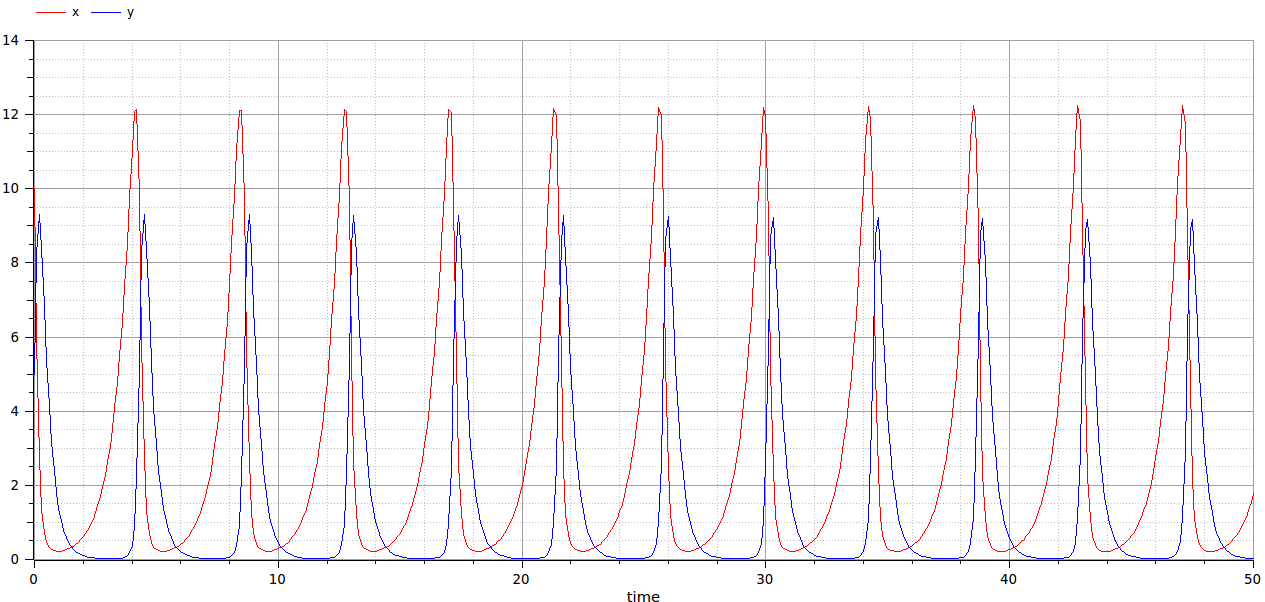
\includegraphics[scale=0.18]{Selection_056.png}	&		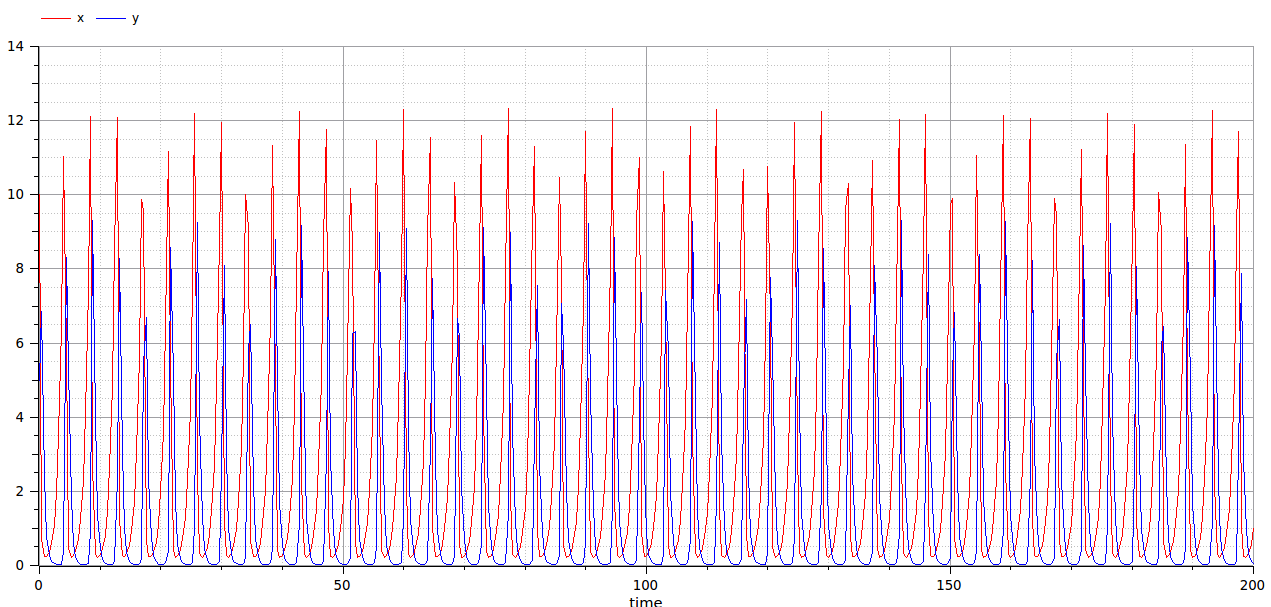
\includegraphics[scale=0.18]{Selection_057.png}\\
		\footnotesize(a)	&	\footnotesize(b)\\

	\end{tabular}
\end{center}
\vspace{-0.5cm}

\caption{DASSL: (a) 50 second simulation (b) 200 second simulation.}
\end{figure}




\subsection{Euler}

Euler solvers cannot solve this model for more than 23 seconds. The solver incorrectly calculates the values of the state variables when the numberOfIntervals are not explicitly increased to a large number. When this is not done, the model breaks as shown in the graph below. Increasing the numberOfIntervals increases the computational time significantly, but making this number really large will increase the accuracy.

\begin{figure}[htbp]
\begin{center}
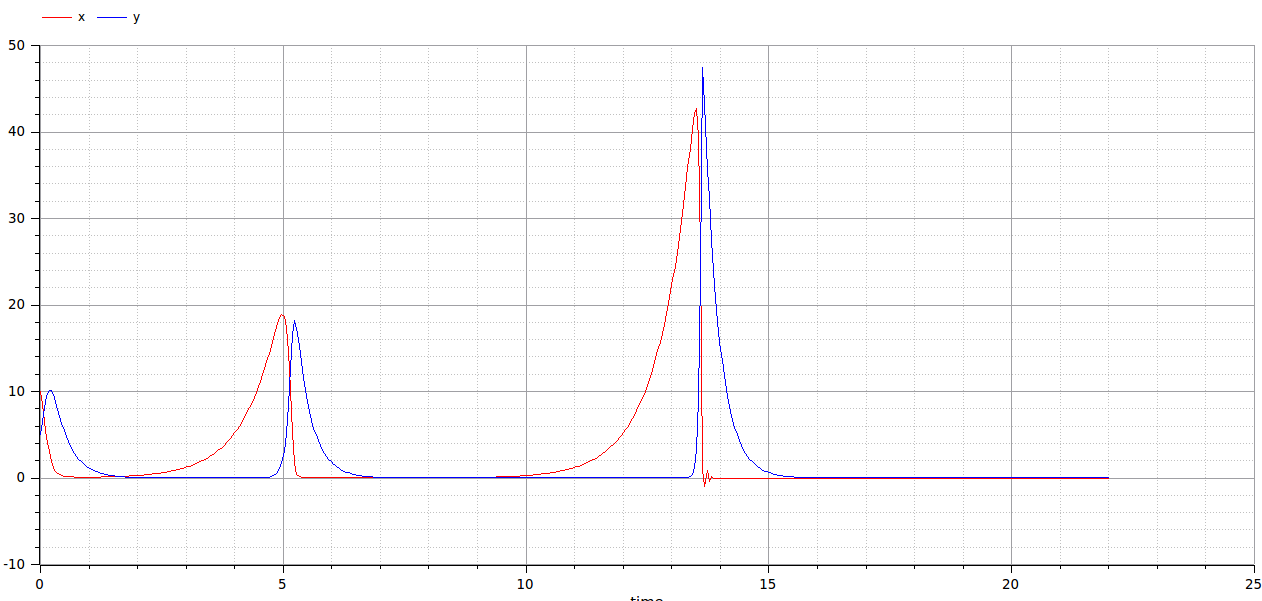
\includegraphics[scale=0.26]{Selection_055.png}
\end{center}
\vspace{-0.5cm}

\caption{Euler: 22 second simulation.}
\end{figure}


\subsection{LIQSS}

Our Linearly Implicit Quantized State Systems (LIQSS) solver has some preliminary results which we can report. This solver is still very much under development at this stage. We do, however, have some promising results. One of the current issues is that oscillating state variables lose accuracy as time increases.

\begin{figure}[htbp]
\begin{center}
\begin{tabular}{cc}
		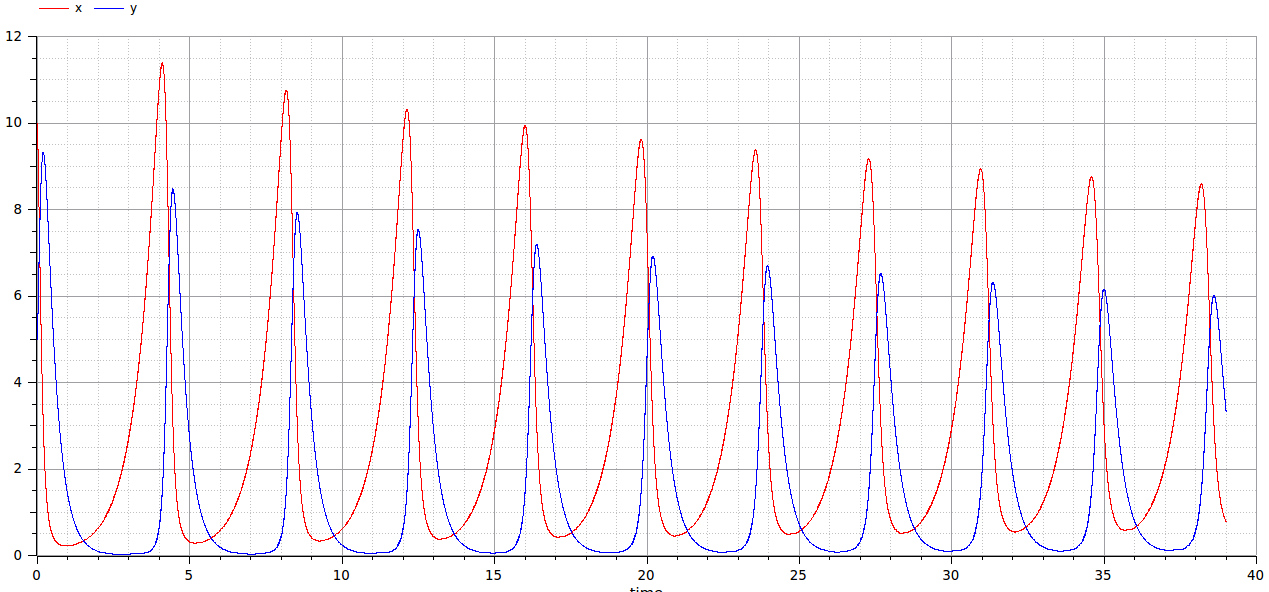
\includegraphics[scale=0.18]{Selection_059.png}	&		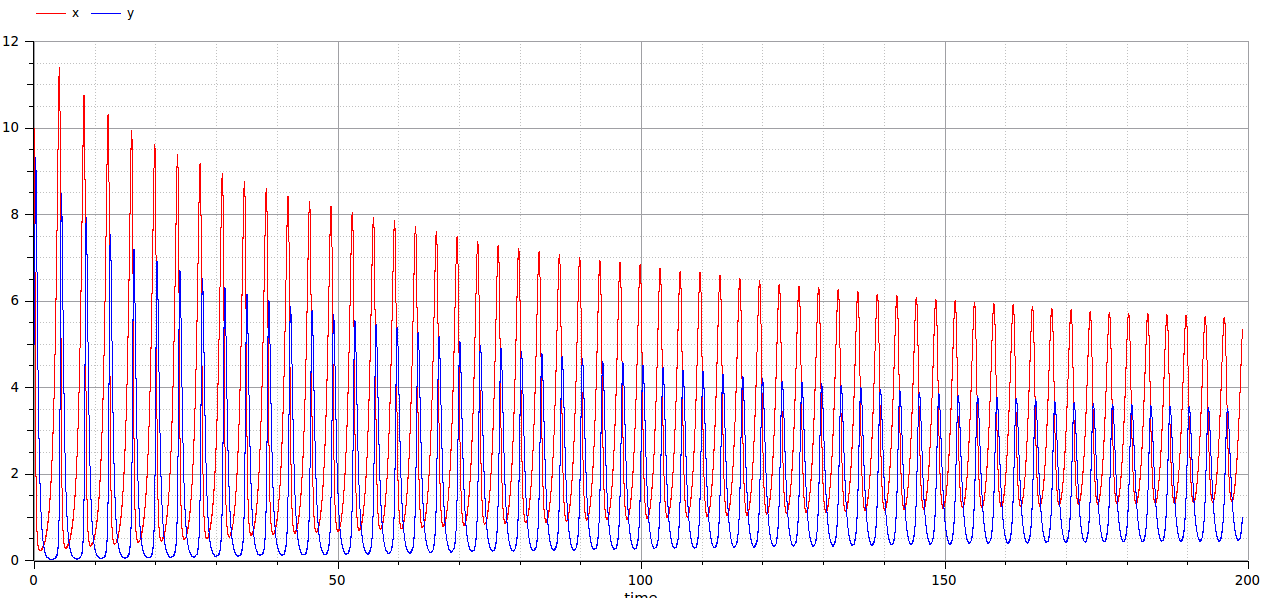
\includegraphics[scale=0.18]{Selection_058.png}\\
		\footnotesize(a)	&	\footnotesize(b)\\
						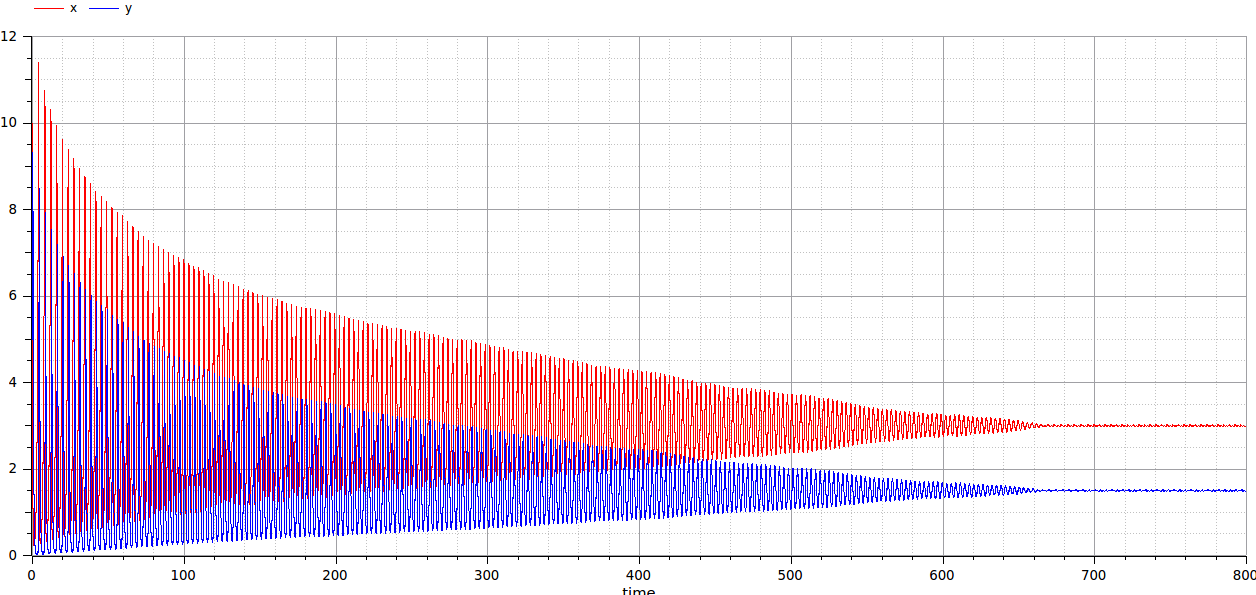
\includegraphics[scale=0.18]{Selection_061.png}	\\
		\footnotesize(c)	\\
	\end{tabular}
\end{center}
\vspace{-0.5cm}

\caption{LIQSS: (a) 40 second simulation (b) 200 second simulation  (c) 800 second simulation. \\ In this case $\Delta Q_x =\Delta Q_y =0.01$.}
\end{figure}

Currently, the most significant element influencing the computation time of the LIQSS solver is step size $\Delta Q_i$ for each state variable $i$. This value is obtained by multiplied by the nominal value of each state variable by a small constant. The smaller we set $\Delta Q_i$ the more accurate our results become, yet the simulation time necessarily increases due to more step updates.

\section{Other solvers}

A summary of the remaining solvers in OpenModelica will be considered.

\begin{table}[htbp]
	\centering%\footnotesize
		\begin{tabular}{ccm{12cm}}
    \topline	\headcol
    Solver&& Description\\\midline
    Radau5 && This solver is able to simulate the Lotka-Volterra. The results are accurate.\\\rowcol
    Radau3 && Similar to Radau5, just not as accurate.\\\rowcol
    Rungekutta && Solves really well when the simulation time is short. Looses some accuracy when the simulation time increases.\newline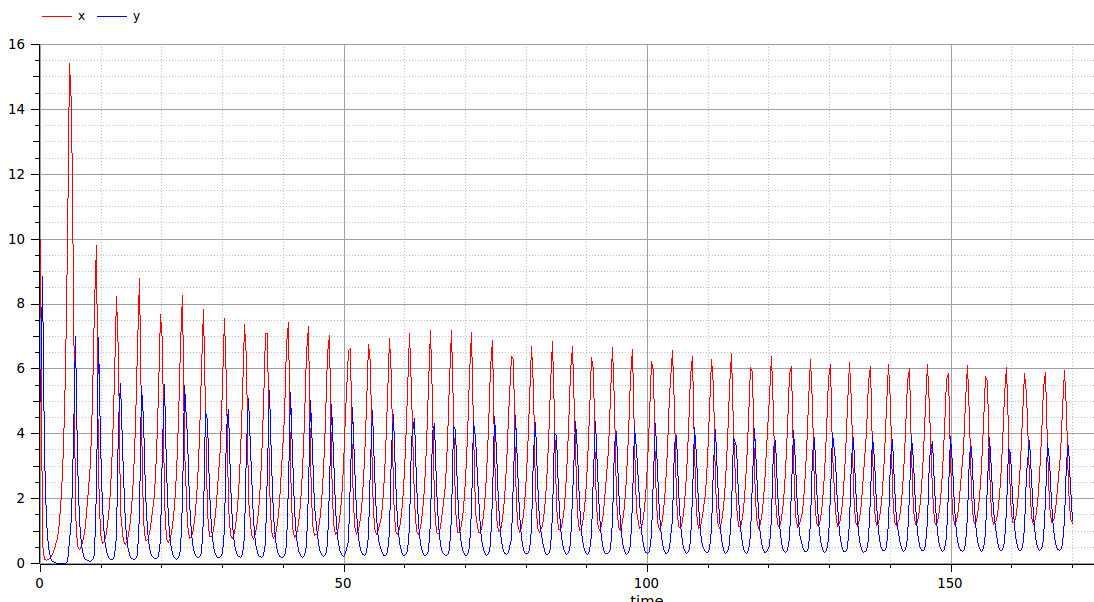
\includegraphics[scale=0.3]{rk.png}\\
    Remaining solvers &&The other solvers include: impeuler,       trapezoid, lobatto4,  lobatto6, symEuler,  symEulerSsc and    heun.

    These solver are all very similar. There is always some point when setting the simulation time at which the solvers are unable to simulate the model when the numberOfIntervals are not increased, thus increasing the simulation time. Some of these solvers behave more like he Euler solver, in that they quickly very inaccurate results or that they are unable to solve the ODE system for an extended period of time. \\\bottomline
    \end{tabular}
    \end{table}

\section{Results}



Some execution time comparisons on two systems have been done. The tolerance of the DASSL solver was set at $1e^{-9}$. For the LIQSS solver the tolerances varied between $\Delta Q_i =0.1$ and $0.001$.

\begin{table}[htbp]
	\centering%\footnotesize
		\begin{tabular}{ccccccccc}
    \topline	\headcol
   sim time & \multicolumn{3}{c}{Lotka-Volterra} \\\headcol
   & DASSL & LIQSS $\Delta Q_i =0.1$ & LIQSS $\Delta Q_i =0.001$ \\\midline
   10& 0.524657877 & 0.584381149&1.099513323\\\rowcol
   100& 0.527889395& 0.969856535&3.639154603\\
   500& 0.562121132& 1.810497473&6.548079135\\\bottomline
  \headcol
   sim time & \multicolumn{3}{c}{Van der Poll} \\\headcol
   & DASSL & LIQSS $\Delta Q_i =0.1$ & LIQSS $\Delta Q_i =0.001$ \\\midline
   10& 0.532238764 & 0.536072432&0.681485771\\\rowcol
   100& 0.541245455& 0.521799247&1.732732925\\
   500& 0.549132642& 0.545967053&6.835242508\\\bottomline
    \end{tabular}
    \caption{Simulation times in seconds.}
    \end{table}



%     \subsubsection{Stiff System 1}
%     \begin{align*}
% \frac{dx}{dt}  &= 0.01y \\
% \frac{dy}{dt}  &= -100x -100y +2\,020
% \end{align*}
% with $x=20, y =0$.
%
%     \subsubsection{Stiff System 2}
%     \begin{align*}
% \frac{dx}{dt}  &= 0.013x - 1\,000xz \\
% \frac{dy}{dt} & = -2\,500yz\\
% \frac{dz}{dt}  &= 0.013x - 1\,000xz - 2\,500yz
% \end{align*}
% with $x=1, y =1, z=0$.

The significance of the tolerance in the LIQSS solver can see in the graphs below.

\begin{figure}[htbp]
\begin{center}
\begin{tabular}{cc}
		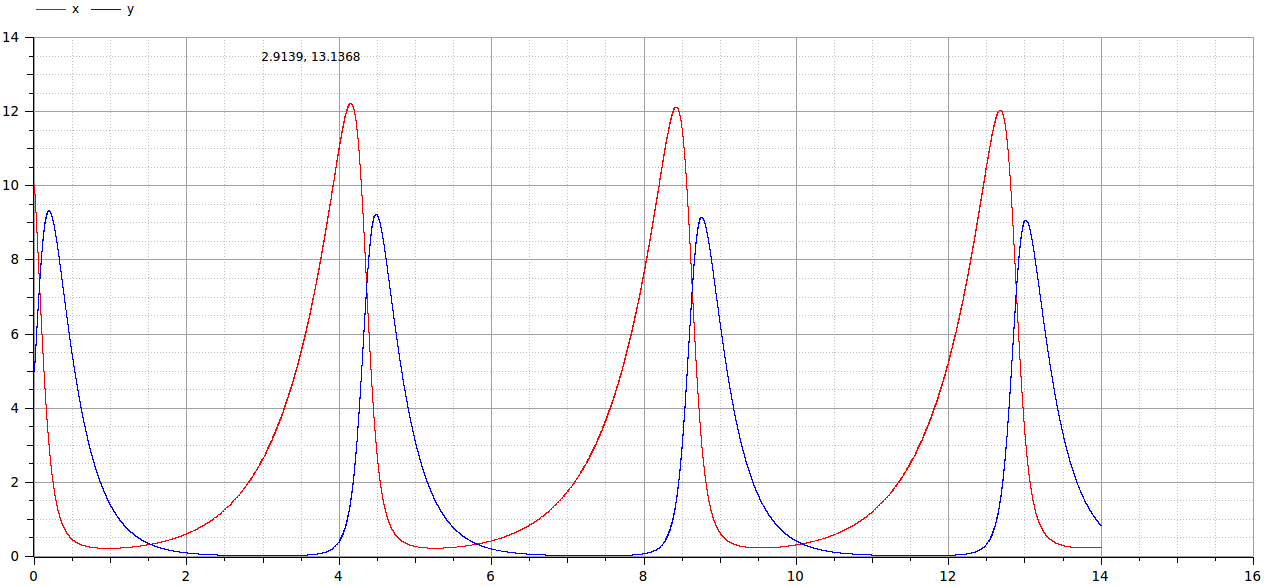
\includegraphics[scale=0.34]{Selection_066.png}	\\	\footnotesize(a)\\	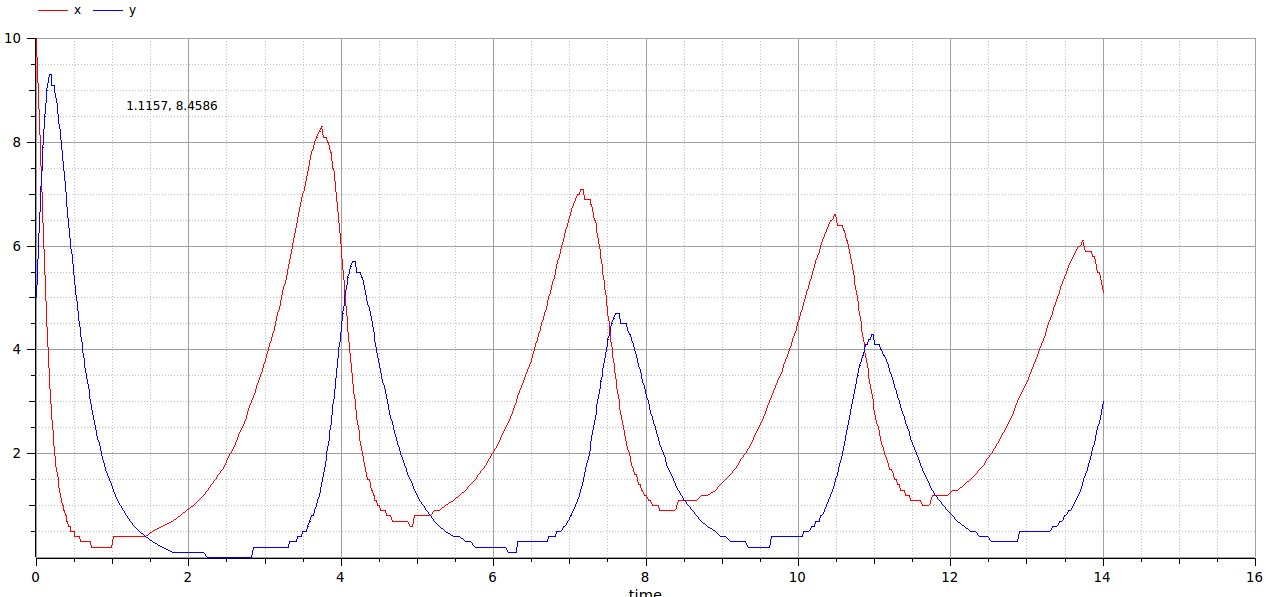
\includegraphics[scale=0.34]{Selection_067.png}\\
	\footnotesize(b)
	\end{tabular}
\end{center}
\vspace{-0.5cm}
\caption{Lotka-Volterra: (a) LIQSS with $\Delta Q_i =0.001$  (b) LIQSS with $\Delta Q_i =0.1$ }
\end{figure}

The LIQSS solver was, however, much more accurate when solving the Van der Poll model and did not converge to zero at all.

\section{Conclusion}

Although there are still many issues to resolve within the current LIQSS solver in OM the solver does not break during execution, which is in contrast to many of the other solvers. The main issues to currently address are:
\begin{itemize}
 \item Ensure event handling occurs when expected and that events are triggered correctly.
 \item Standardize tolerances on this solver and ensure that state variable do not deviate significantly from the expected values.
 \item Optimize implementation code of the solver.
 \item Gauge the possibility of extending the current solver to implement higher order LIQSS solvers.
\end{itemize}

\end{document}